\documentclass[a4paper]{report}
\usepackage[textwidth=17cm, textheight=25cm]{geometry}
\usepackage{verbatim}

\usepackage[utf8]{inputenc}
\usepackage[ngerman]{babel}
\usepackage[pdftex]{hyperref}

\usepackage{amsmath, amssymb}
\usepackage{enumerate}
\usepackage{multicol} % multiple collums in enumerate
\usepackage{graphicx}
\usepackage{tabu}
\title{C++ in Übersichten \\ \medskip \large Material zum C++ Kurs}
\author{Maximilian Starke \\ Student der TU Dresden \\ Fakultät Informatik}
\date{\today}

%\usepackage[thmmarks,amsmath,hyperref,noconfig]{ntheorem}
\usepackage{listings}
\usepackage{fancybox}
\input{syntax.tex}
\usepackage{tikz}
\usepackage{rail}


  % erlaubt es, Sätze, Definitionen etc. einfach durchzunummerieren.
%\newtheorem{satz}{Satz}[section] % Nummerierung nach Abschnitten
%\newtheorem{proposition}[satz]{Proposition}
%\newtheorem{kor}[satz]{Korollar}

% --------------------------------------math
%\theorembodyfont{\upshape}
%\newtheorem{beispiel}[satz]{Beispiel}
%\newtheorem{bemerkung}[satz]{Bemerkung}
%\newtheorem{definition}[satz]{Definition} %[section]

%\theoremstyle{nonumberplain}
%\theoremheaderfont{\itshape}
%\theorembodyfont{\normalfont}
%\theoremseparator{.}
%\theoremsymbol{\ensuremath{_\blacksquare}}
%\newtheorem{beweis}{Beweis}
%\qedsymbol{\ensuremath{_\blacksquare}}

%------------------------------------------------------
\usepackage{tikz}
\usetikzlibrary{shapes,arrows}

\usetikzlibrary{%
	arrows,%
	shapes.misc,% wg. rounded rectangle
	shapes.arrows,%
	chains,%
	matrix,%
	positioning,% wg. " of "
	scopes,%
	decorations.pathmorphing,% /pgf/decoration/random steps | erste Graphik
	shadows%
}


\usepackage{caption}
\DeclareCaptionFont{white}{\color{white}}

\usepackage{xcolor}
\usepackage{listings}
\usepackage{tcolorbox}
\tcbuselibrary{listings}


\begin{document}

\maketitle

\section*{Vorwort}
Dieses Skript \textbf{C++ in Übersichten} enthält Material zum C++ Kurs, den ich im Sommersemester 2017 halte (\url{ifsr.de/kurse})
Das Skript wird parallel zum Kurs erstellt und erweitert. Es besteht daher momentan noch als Entwurf.

Das Skript dient vordergründig als Nachschlagewerk für den C++ Kurs und besteht im Wesentlichen aus vier Kapiteln zu Einrichtung, Datentypen, strukturierter Programmierung und Randfeatures. Dabei wurde in erster Linie eine Einteilung nach logischen Zusammenhängen der Sprache C++ angestrebt, zweitrangig nach pädagogisch sinnvoller Reihenfolge. Das stellt mehr oder weniger eine hinreichende und zugleich notwendige Bedingung für die parallele Abarbeitung von Kapitel 2 und 3 dar, da Kenntnisse über Datentypen und Mechanismen strukturierter Programmierung an vielen Stellen wieder eine Einheit bilden und ineinander greifen.

\tableofcontents

\chapter{Einrichtung}

\section{ISO C++}

\subsection{Allgemeines}
\begin{itemize}
\item ab 1979 von Bjarne Stroustrup bei AT\&T entwickelt als Erweiterung der Programmiersprache C
\item später von ISO genormt
\vspace{2ex}
\item effizient und schnell - Schnelligkeit eines der wichtigsten Designprinzipien von C++
\item hohes Abstraktionsniveau u.a. durch Unterstützung von OOP
\item ISO Standard beschreibt auch eine Standardbibliothek
\item C++ ist \textbf{kein} echtes Superset von C (siehe stackoverflow.com, \dots)
\item C++ ist (wie C) \textbf{case sensitive}
\vspace{2ex}

\item Paradigmen:
	\begin{itemize}
		\item \textbf{generisch} (durch Benutzung von Templates, automatische Erstellung multipler Funktionen für verschiedene Datentypen)
		\item \textbf{imperativ} (Programm als Folge von Anweisungen, Gegenteil von deklarativ siehe Haskell und Logikprogrammierung)
		\item \textbf{objektorientiert} (Klassen, Objekte, Vererbung, Polymorphie, Idee: Anlehnung an Realität)
		\item \textbf{prozedural} (Begriff mit verschiedenen Bedeutungsauffassungen, Unterteilung des Programms in logische Teilstücke (Prozeduren), die bestimmte Aufgaben / Funktionen übernehmen)
		\item \textbf{strukturiert} (prozedural und Teilung in Sequenz, Verzweigung, Wiederholung, \dots )
		\item \textbf{funktional} (ab C++11, Definitionskleinkram, siehe Wikipedia, Programm als verschachtelter [...] Funktionsaufruf 	organisierbar, eher typisch für Haskell o.ä.)
	\end{itemize}
\end{itemize}

\subsection{Versionen}
\begin{itemize}
	\item C++98
	\item C++03
	\item C++11
	\subitem wesentliche Neuerungen. Einführung von constexpr, Elementinitialisierer, ... Neue Bedeutung des Schlüsselworts auto \hspace{3cm} \# Referenzen ergänzen %#####
	\item C++14
	\subitem aufweichung der constexpr Bedingungen.
	\item C++17
	\subitem soll 2017 vollendet werden.
\end{itemize}

\section{Dateien in einem C++ Projekt}
\begin{center}
\begin{tabular}{|c|c|p{8.5cm}|}
	\hline
	Dateiendung & Bezeichnung & Inhalt \\
	\hline
	(*.cpp) (*.cc) & Quelldatei & Funktionsimplementation, Klassenimplementation, \newline Berechnungen bzw. eigentliche Arbeit erledigen \\ \hline
	(*.h) & Headerdatei & Funktionsdeklaration, Klassendefinition, \newline Bezeichner öffentlich bekannt machen \\
	\hline
	(*.o) & Objektdatei & Objektcode (Maschinencode) einer Übersetzungseinheit\\
	\hline
	(*.exe) (*.out) & ausführbare Datei & fertiges Programm \\
	\hline \hline
	(*.sln) (*.pro) (*.vcxproj) & "Projektdatei" & IDE Einstellungen (oder ähnliches) \newline IDE-spezifische Namen und Verwendung\\
	\hline \hline
	(*.res) & Ressourcendatei & multimediale Inhalte\\
	\hline
\end{tabular}

\vspace{4ex}

% Define block styles
\tikzstyle{block} = [rectangle, draw, fill=blue!40, 
text width=7em, text centered, rounded corners, minimum height=5em, node distance= 4.5cm, line width = 2pt]


\tikzstyle{cblock} = [rectangle, draw, fill=blue!40, 
text width=7em, text centered, rounded corners, minimum height=5em, node distance= 3.0cm, line width = 2pt]


\tikzstyle{line} = [draw, -latex', line width = 4pt]


\tikzstyle{cloud} = [draw, ellipse,fill=red!40, node distance=3cm, line width = 2pt,
minimum height=3em]

{\large

\begin{tikzpicture}[node distance = 3cm, auto]
    % Place nodes
    \node [cloud] (pc) {Precompiler};
    
    \node [block, left of=pc] (cpp) {*cpp, *.c};
    \path [line] (cpp) --(pc);
    
    \node [block, right of=pc] (h) {*.h};
    \path [line] (h) --(pc);
    
    \node [cblock, below of=pc] (cpp2) {cpp without \#precompiler instruction};
    \path [line, below of = cpp2] (pc) -- (cpp2);
    
    \node [cloud, below of = cpp2] (c) {Compiler};
    \path [line] (cpp2) -- (c);
    
    \node [cblock, below of = c] (o) {*.o};
    \path [line] (c) -- (o);
    
    \node [cloud, below of = o] (l) {Linker};
    \path [line] (o) -- (l);
    
    \node [block, left of =o] (lo) {another\\ *.o};
    \path [line] (lo) -- (l);
    
    \node [block, right of = o] (ro) {another\\ *.o};
    \path [line] (ro) -- (l);
    
    \node [cblock, below of = l] (exe) {*.exe, *.out};
    \path [line] (l) -- (exe);
     
    \node [block, right of = exe] (lib) {*.lib, *.dll};
    \path [line] (l) -- (lib); 

\end{tikzpicture}
}
\end{center}


\section{Compiler}
\begin{center}
\begin{tabular}{|c|l|}
	\hline
	\textbf{Compiler} & \textbf{Plattform} \\ \hline \hline
	GCC/g++ & Windows, Linux, Mac, Unix-like \\ \hline
	Clang & Unix-like, Mac, Windows, Linux \\ \hline
	Intel-C++ & Linux, Windows, Mac \\ \hline
	VC++ & Windows \\ \hline
\end{tabular}
\end{center}
Das nun folgende Listing zeigt, wie ein C++ Quellcode, der als Datei vorliegt, "`per Hand"' mit Kommandozeile unter Nutzung des Compilers (hier g++) übersetzt werden kann. Beim Aufruf des Compilers wurden hier noch einige Flags gesetzt, nämlich \texttt{-Wall}, um \textbf{sinnvolle Warnungen} ausgeben zu lassen, und \texttt{-pedantic}, um \textbf{vom C++ Standard geforderte Warnungen} erscheinen zu lassen. Außerdem wurde der C++ Standard (Version) gesetzt.

\begin{tcblisting}{colback=yellow!10,colframe=yellow!40!black,listing only,
		title=Nutzung von g++ mittels Powershell, fonttitle=\bfseries}
PS A:\> cd .\example\
PS A:\example> ls


Verzeichnis: A:\example


Mode                LastWriteTime         Length Name
----                -------------         ------ ----
-a----       02.04.2017     08:38             87 hello_world.cpp


PS A:\example> type .\hello_world.cpp
#include <iostream>

int main(){
	std::cout << "Hello World";
	return 0;
}

PS A:\example> g++ -o programm hello_world.cpp -Wall -pedantic -std=c++11
PS A:\example> ls


Verzeichnis: A:\example


Mode                LastWriteTime         Length Name
----                -------------         ------ ----
-a----       02.04.2017     08:38             87 hello_world.cpp
-a----       02.04.2017     09:12          48650 programm.exe


PS A:\example> .\programm.exe
Hello World
PS A:\example>
\end{tcblisting}

Eine kleine Anmerkung zu Bezeichnungen, die mit Compilern zu tun haben, möchte ich an dieser Stelle noch loswerden, da hier immer eine kleine Verwechslungsgefahr besteht. Die \textbf{GCC} \textit{(GNU Compiler Collection)} ist eine Compilersammlung mit Compilern zu C, C++ und einigen weiteren. Dagegen ist der \textbf{gcc} (klein geschrieben) der C-Compiler der Sammlung und \textbf{g++} der C++-Compiler.

Um auf Ihrem Betriebssystem einen C++ Compiler zum Laufen zu bringen, haben Sie meist verschiedenste Möglichkeiten.

Um unter \textbf{Linux} GCC zu nutzen, müssen lediglich die entsprechenden Pakete installiert werden, meist ist die GCC sogar schon vorinstalliert.

Unter \textbf{Windows} kann man den von Microsoft bereitgestellten Visual C++ Compiler verwenden, i.d.R. in Verbindung mit einer Installation von Visual Studio (eine IDE für u.a. C++). Die zu installierenden Komponenten bei Visual Studio kann man selbst beim Installationsprozess auswählen, i.A. ist der Speicherverbrauch jedoch relativ groß. Wer auf eine speicherschonende Variante zurückgreifen will oder muss, dem empfehle ich MinGW - eine Portierung der GCC aus dem Hause Linux für Windows. Planen Sie früher oder später Qt-Creator als eine C++-IDE zu installieren, dann können Sie sich einen extra Installation von MinGW im Vorhinein sparen, da QT-Creator MinGW bereits mitinstalliert. Sofern mit der Kommandozeile direkt auf g++ zugegriffen werden soll, ist es unter Windows i.d.R. erforderlich den Pfad der MinGW-Binarys der Systemvariablen \texttt{PATH} hinzuzufügen.

\begin{comment}
\lstdefinestyle{framed}
{
frame=lrb,        
belowcaptionskip=-1pt,
xleftmargin=8pt,
framexleftmargin=7pt,
framexrightmargin=6pt,
framextopmargin=5pt,
framexbottommargin=5pt,
framesep=0pt,
rulesep=0pt,
}

\begin{lstlisting}[style = framed, caption = Nutzung von g++ mittels Powershell]
PS A:\> cd .\example\
PS A:\example> ls


Verzeichnis: A:\example


Mode                LastWriteTime         Length Name
----                -------------         ------ ----
-a----       02.04.2017     08:38             87 hello_world.cpp


PS A:\example> type .\hello_world.cpp
#include <iostream>

int main(){
	std::cout << "Hello World";
	return 0;
}
	
PS A:\example> g++ -o programm hello_world.cpp -Wall -pedantic -std=c++11
PS A:\example> ls


Verzeichnis: A:\example


Mode                LastWriteTime         Length Name
----                -------------         ------ ----
-a----       02.04.2017     08:38             87 hello_world.cpp
-a----       02.04.2017     09:12          48650 programm.exe


PS A:\example> .\programm.exe
Hello World
PS A:\example>
\end{lstlisting}
\end{comment}


\section{IDEs}
\subsection{JA oder NEIN}
\begin{center}
\begin{tabular}{|c||c|}
	\hline
	\textbf{ohne IDE} & \textbf{mit IDE} \\
	\hline \hline
	Compiler, Linker über Shell bedienen	&	Projekteinstellungen \& Buttons \\
	Texteditor				&		in IDE integriert\\
	evtl. make + makefile	&	automatisch generiertes makefile \\
	Dokumentationen & geordneter Menübaum \\
	\hline \hline
	Einarbeitungszeit (??) & Einarbeitungszeit (??) \\
	für kleine und mittelgroße Projekte & kleine, mittlere und große Projekte \\
	\hline
\end{tabular}
\end{center}

\subsection{IDEs im Überblick}
\begin{center}
\begin{tabular}{|c|c|p{10cm}|}
	\hline
	\textbf{IDE} & \textbf{Plattform} & \textbf{Anmerkungen}\\
	\hline
	Eclipse, Netbeans & Java (JVM) & in und für Java geschrieben, unterstützt auch C++ \\
	Qt SDK & WIN, Linux, Mac & bringt umfangreiches Qt-Framework mit für GUIs u.v.m. \\
	Code::Blocks & WIN, Linux, Mac & \\
	\hline
	Visual Studio & Windows & kostenfreie BVersion für den Hausgebrauch: VS Community 2017, sehr umfangreich (Refactoring Tools, Debugger, Laufzeitanalyse, Frameworks wie MFC, ATL, WTL) und damit auch speicherintensiv, zu installierende Features wählbar, benutzt eigenen MS VC++ Compiler\\
	Orwell DEV-C++ & Windows &\\
	\hline
	Geany & Linux, WIN & schlichter Texteditor mit Syntaxhighlighting und diversen Buttons für Compilerausführung, Logausgabe\\
	KDevelop & Linux, WIN & \# \\ %#####
	Anjuta & Linux & \# \\ %#####
	\hline
	XCode & MacOS & "`hauseigene"' IDE von Apple\\
	\hline
	
\end{tabular}

\vspace{4ex}

Auf den Seiten \pageref{begin:ide:picts} bis \pageref{end:ide:picts} finden sich Screenshots einiger IDEs.

\begin{figure}
	\label{begin:ide:picts}
	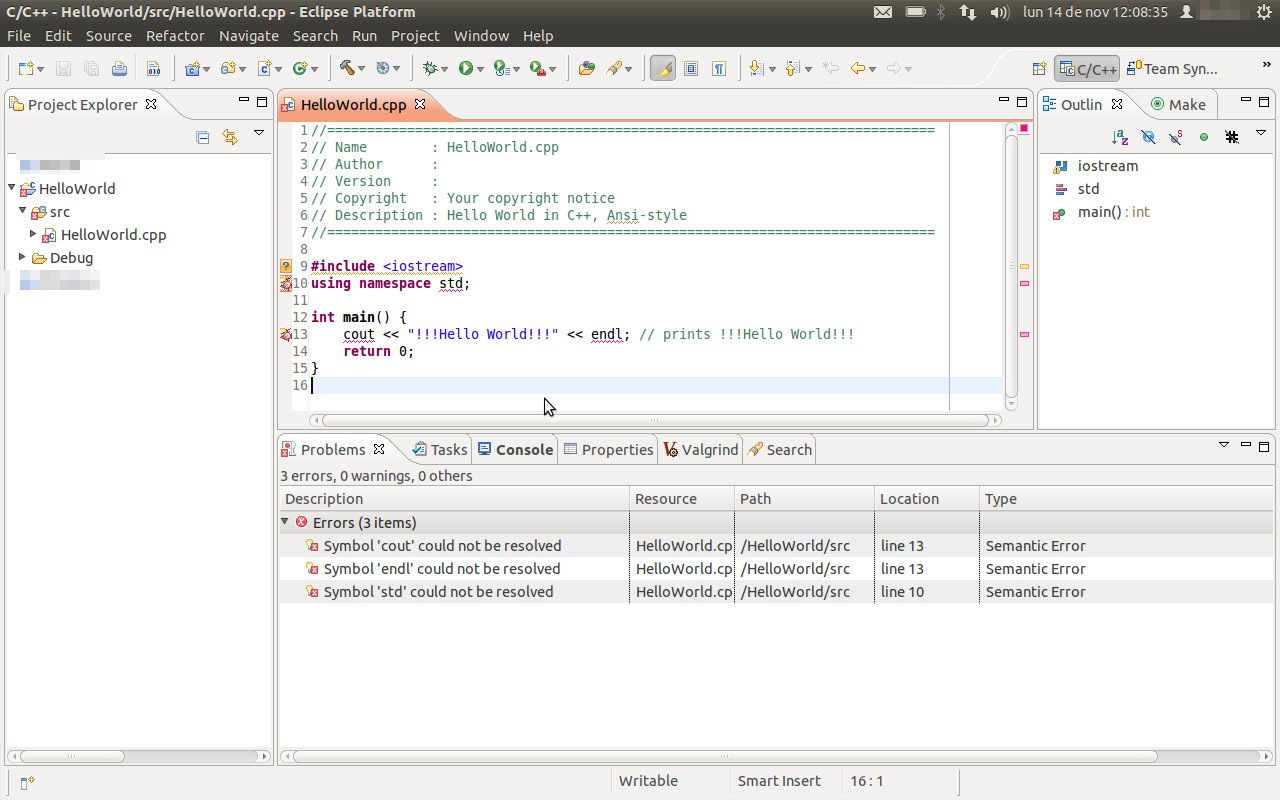
\includegraphics[width = \textwidth]{01/eclipse.jpg}
	\caption{Eclipse mit einem C++ Projekt}
	\url{https://www.eclipse.org/forums/index.php/fa/6135/0/}
	\label{pic:eclipse}
\end{figure}
\begin{figure}
	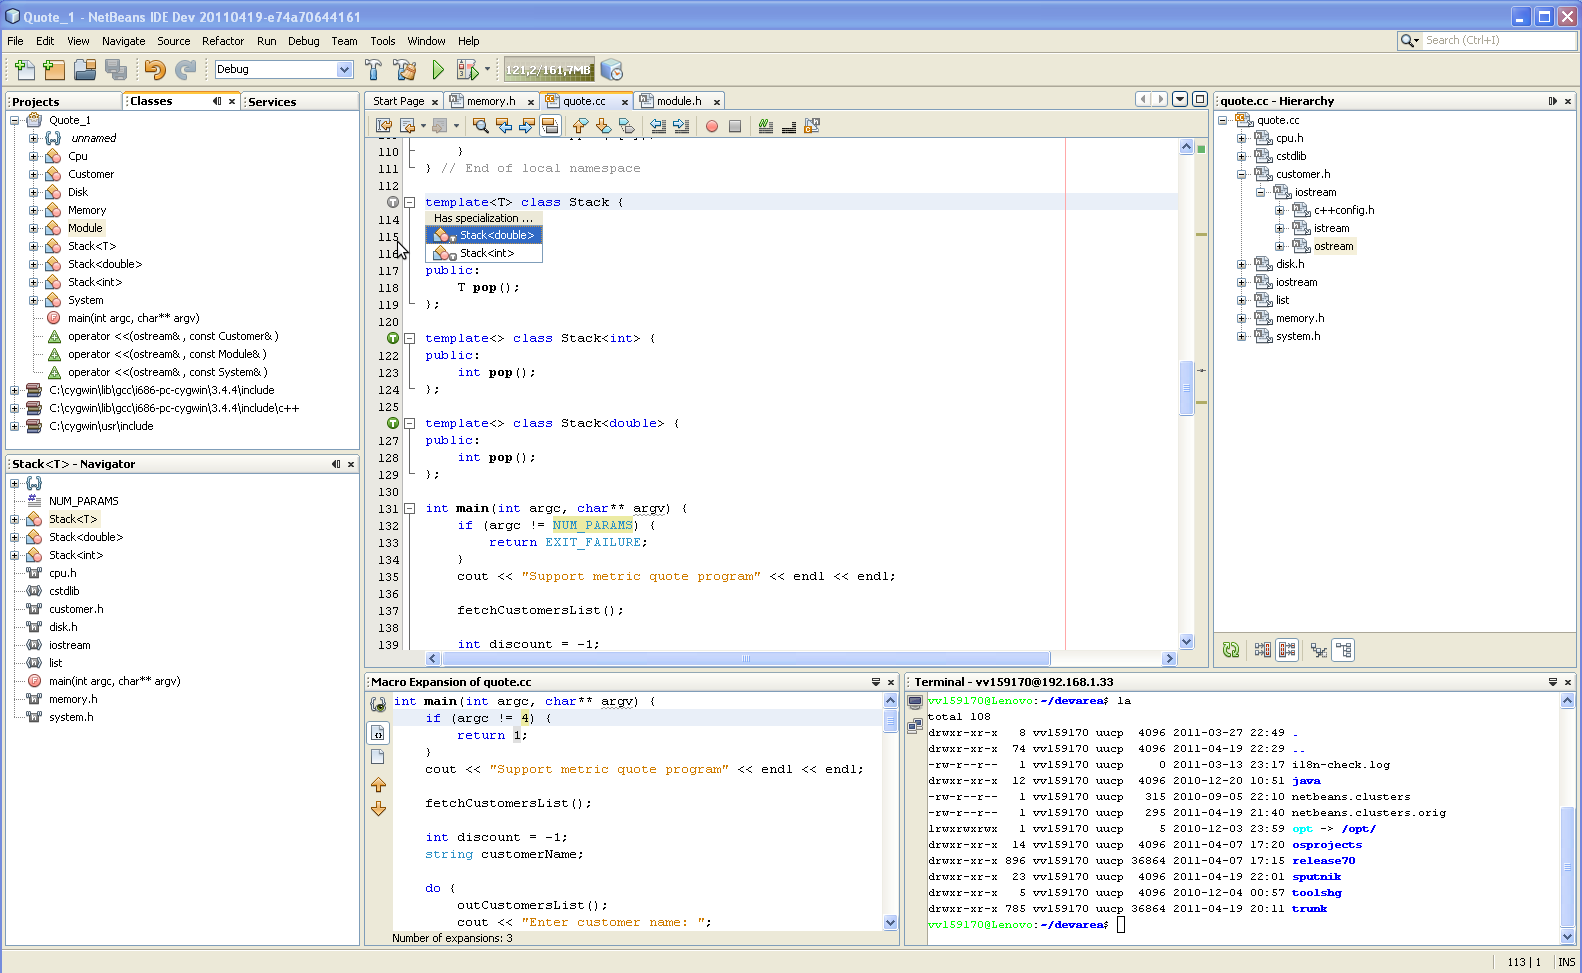
\includegraphics[width = \textwidth]{01/netbeans.png}
	\caption{NetBeans und die Verwendung von C++}
	\url{https://netbeans.org/images_www/v7/screenshots/cnd.png}
	\label{pic:netbeans}
\end{figure}
\begin{figure}
	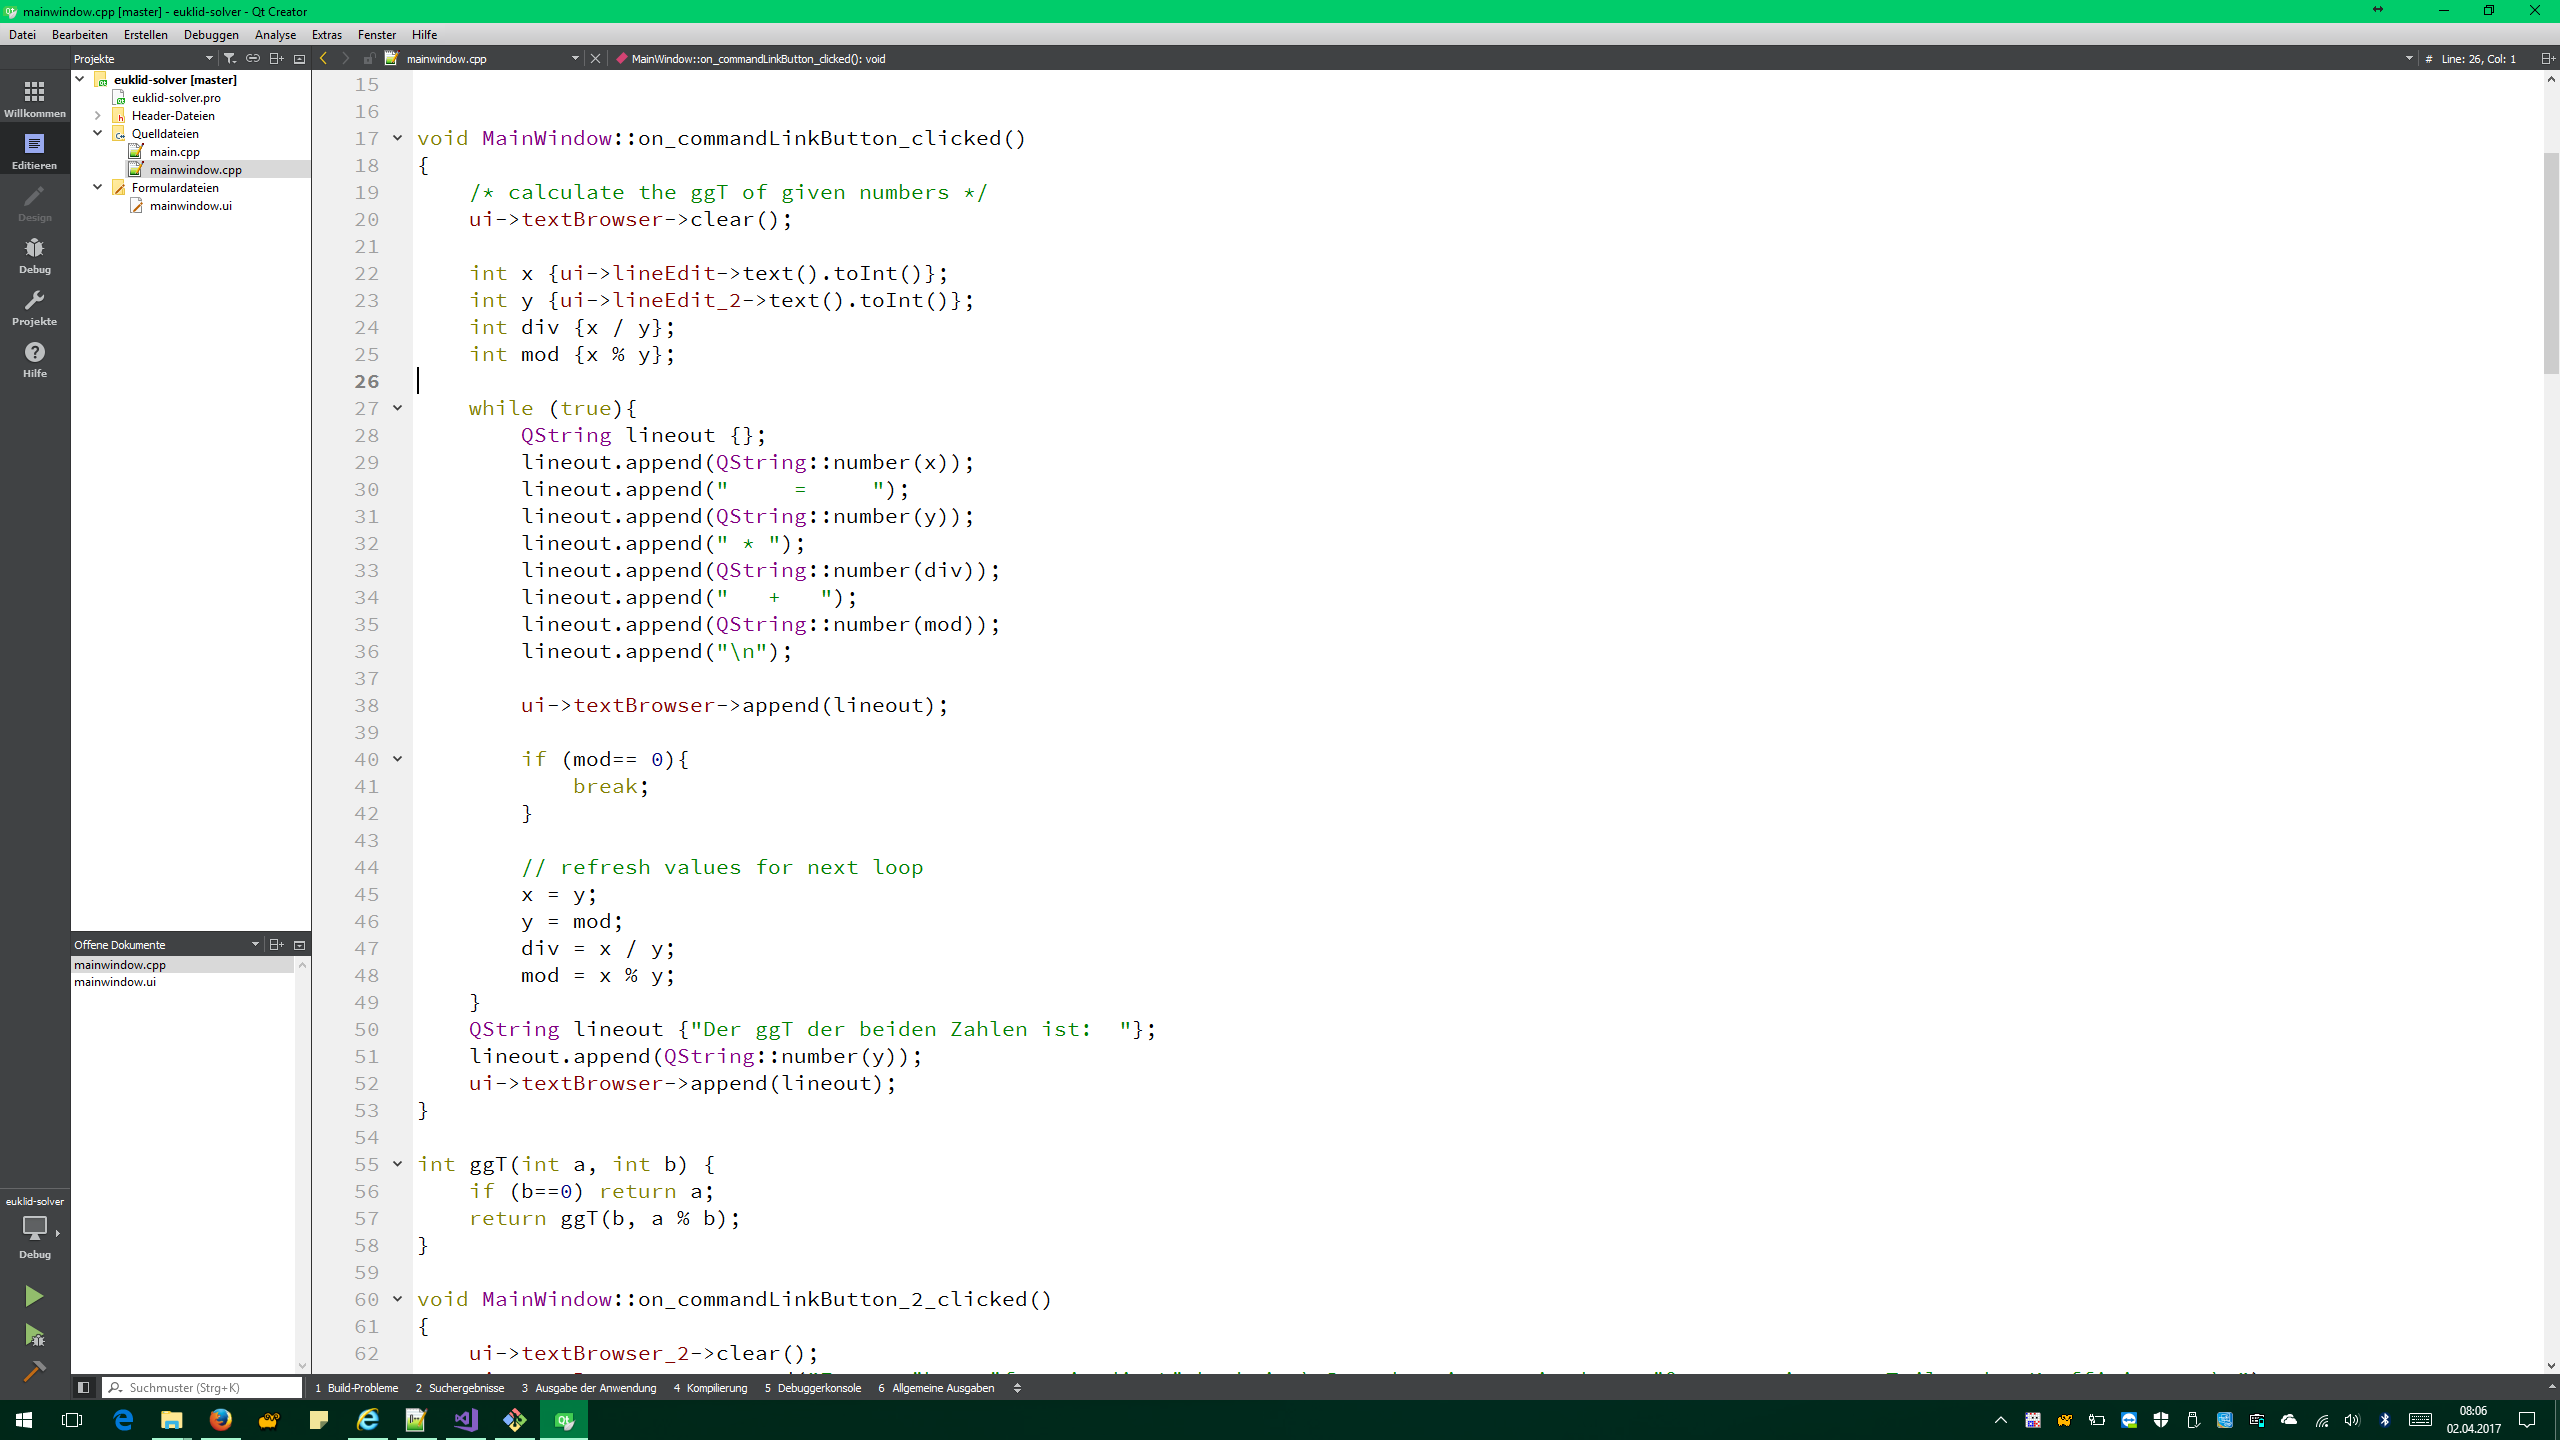
\includegraphics[width = \textwidth]{01/qt_code.png}
	\caption{C++ Code in der QT Creator IDE}
	\label{pic:qt_code}
\end{figure}
\begin{figure}
	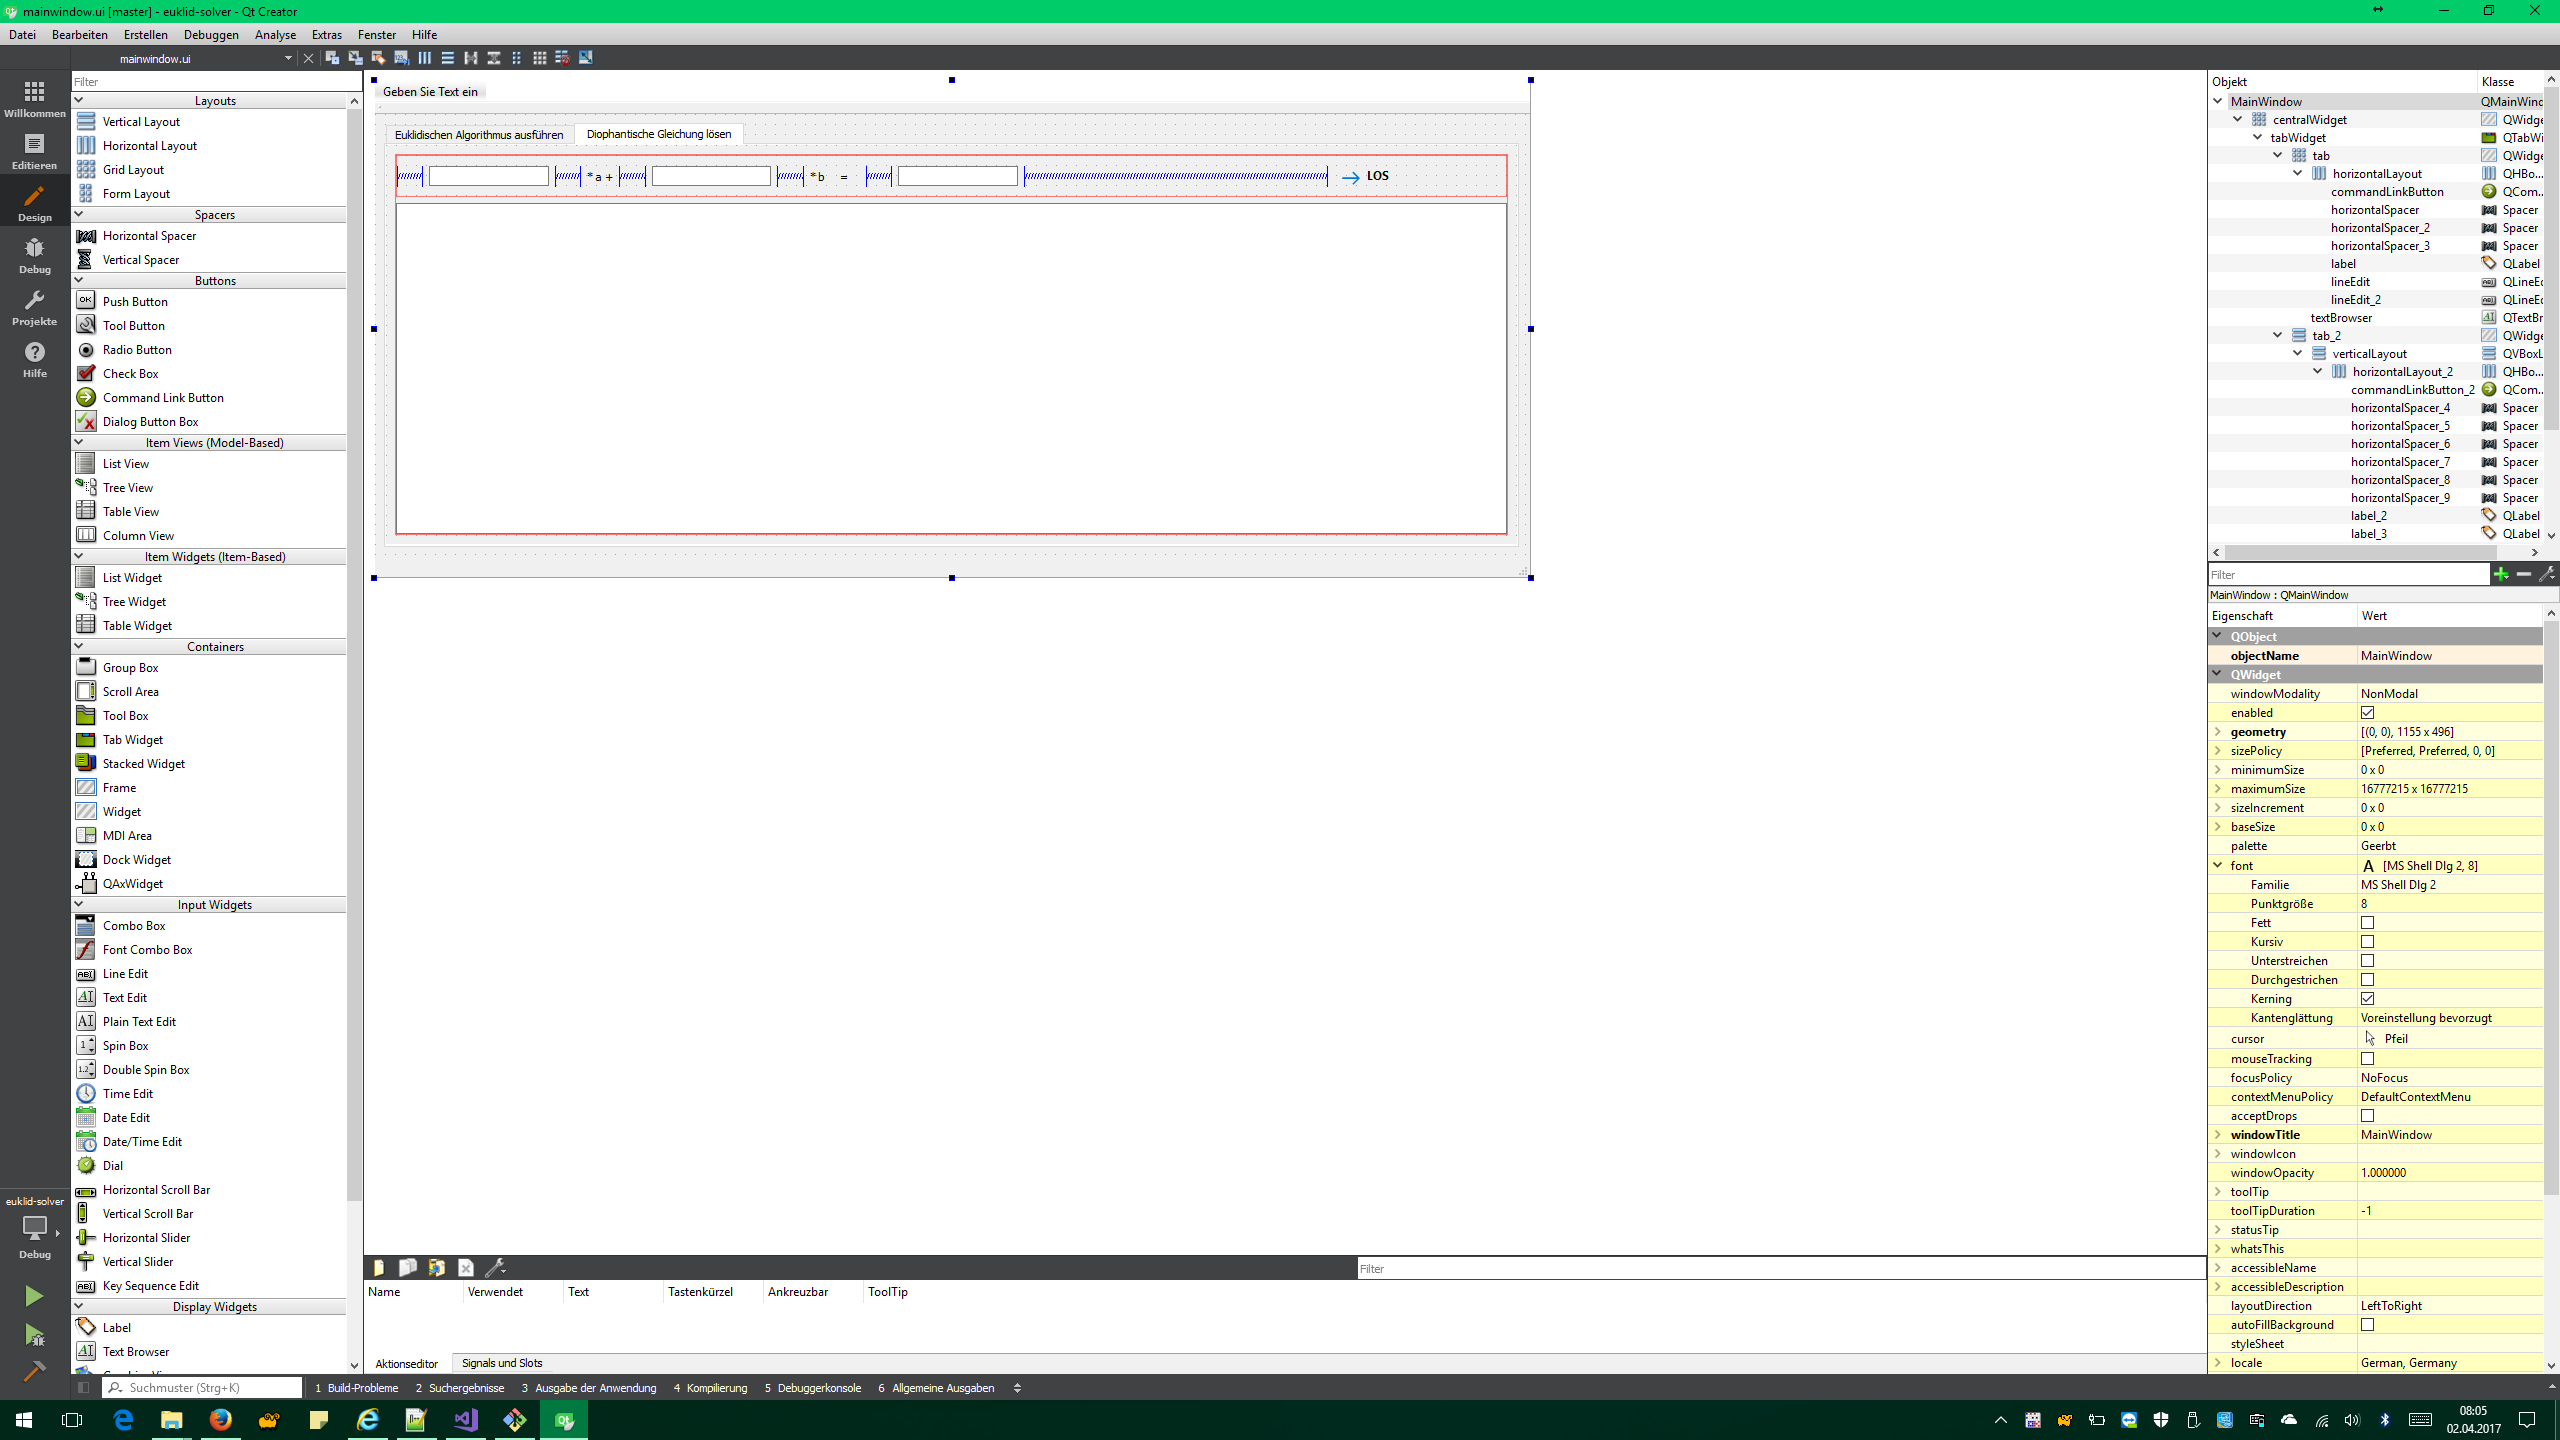
\includegraphics[width = \textwidth]{01/qt_designer.png}
	\caption{Fensterdesign mit QT Creator}
	\label{pic:qt_designer}
\end{figure}
\begin{figure}
	\centering
	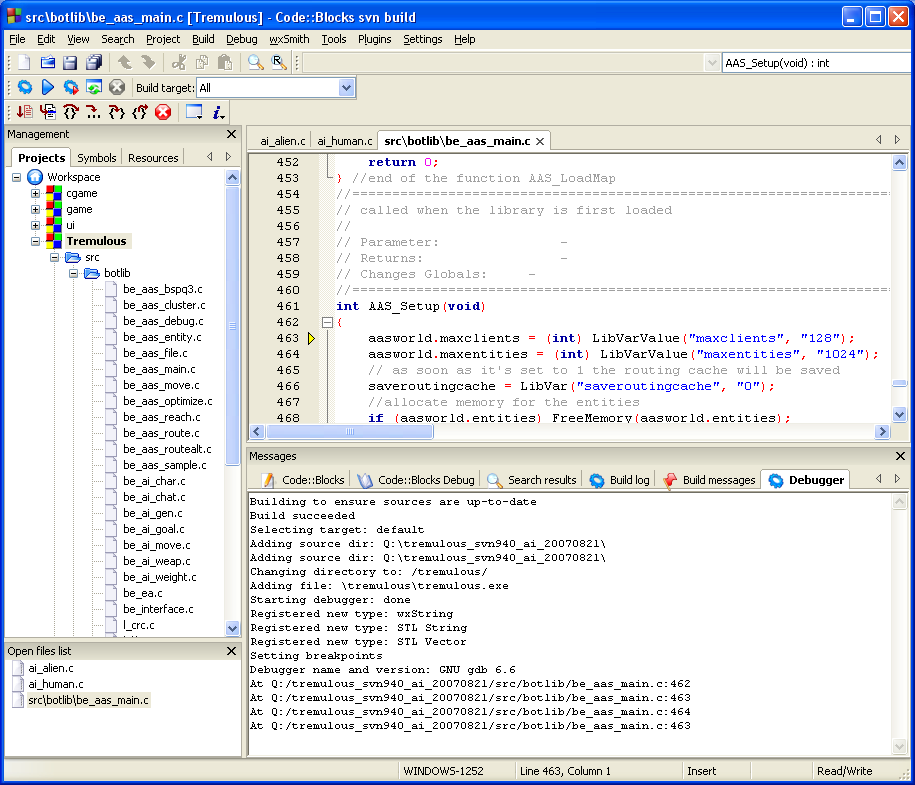
\includegraphics[width = 13cm]{01/codeblocks.png}
	\caption{Code Blocks}
	\label{pic:code::blocks}
	\url{http://www.aftermoon.net/img/20070905_codeblocks_tremulous.png}
\end{figure}
\begin{figure}
	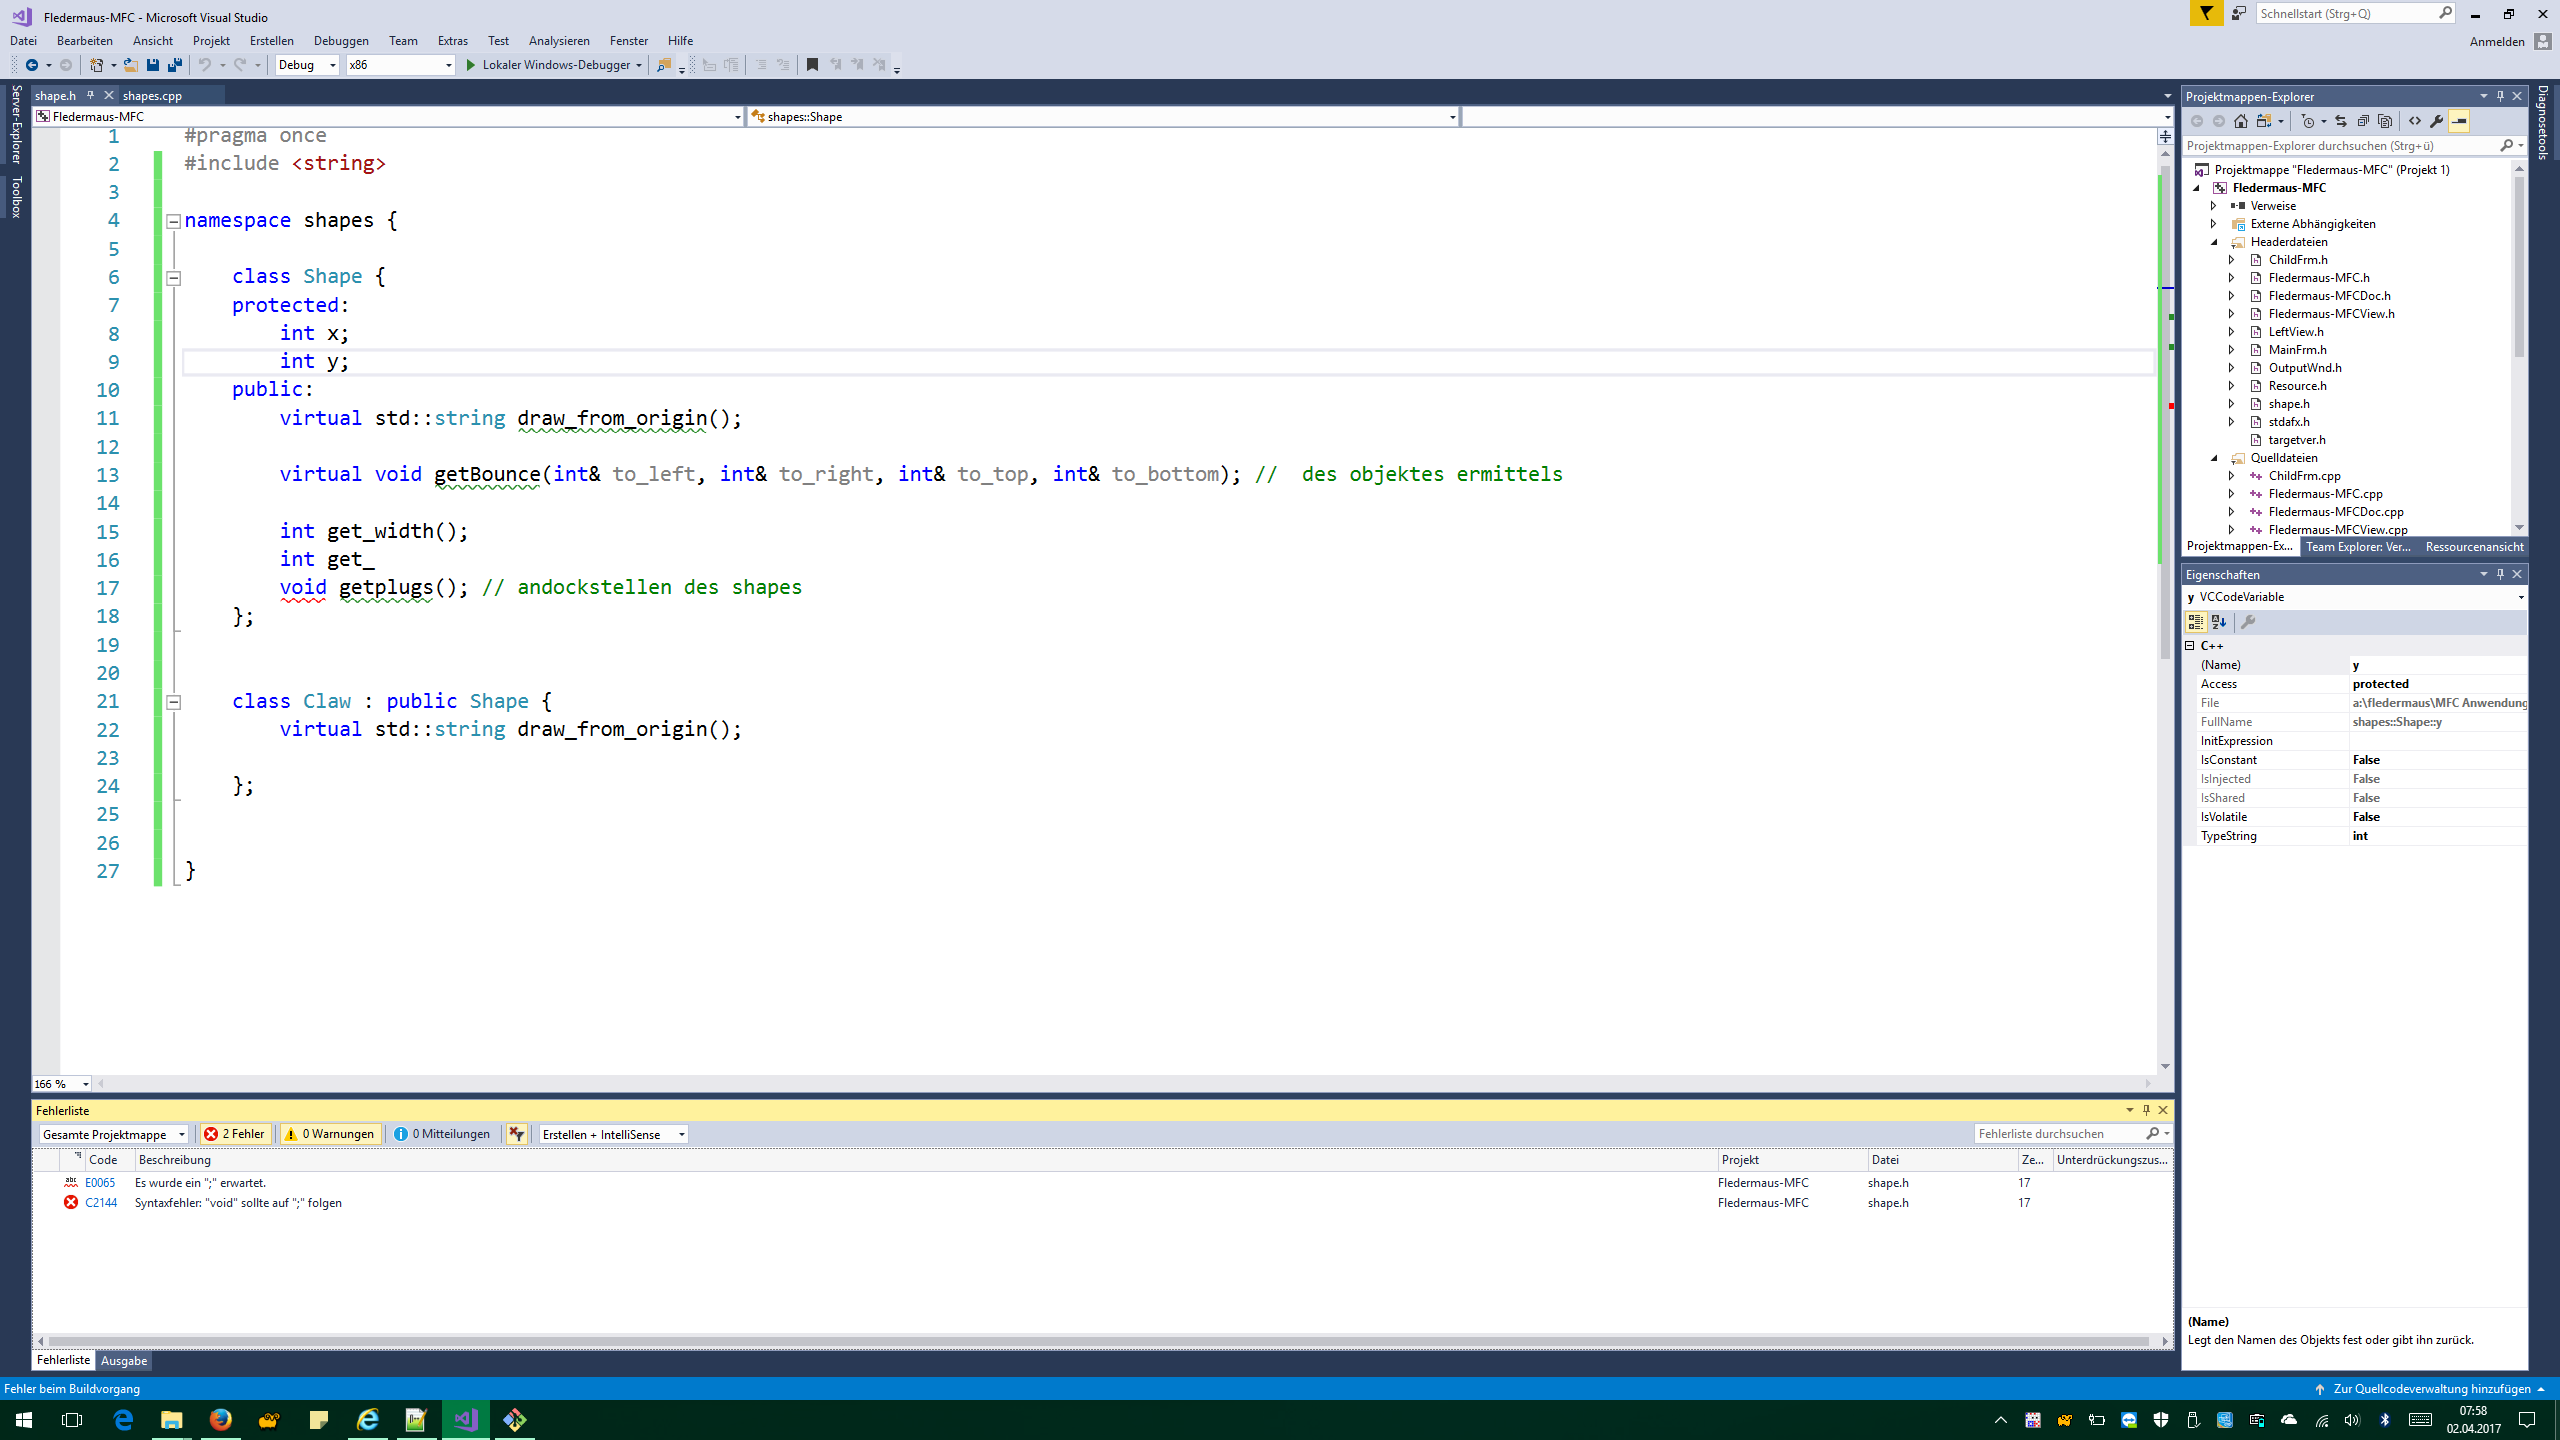
\includegraphics[width = \textwidth]{01/vs.png}
	\caption{Visual Studio Community}
	\label{pic:visualstudio}	
\end{figure}
\begin{figure}
	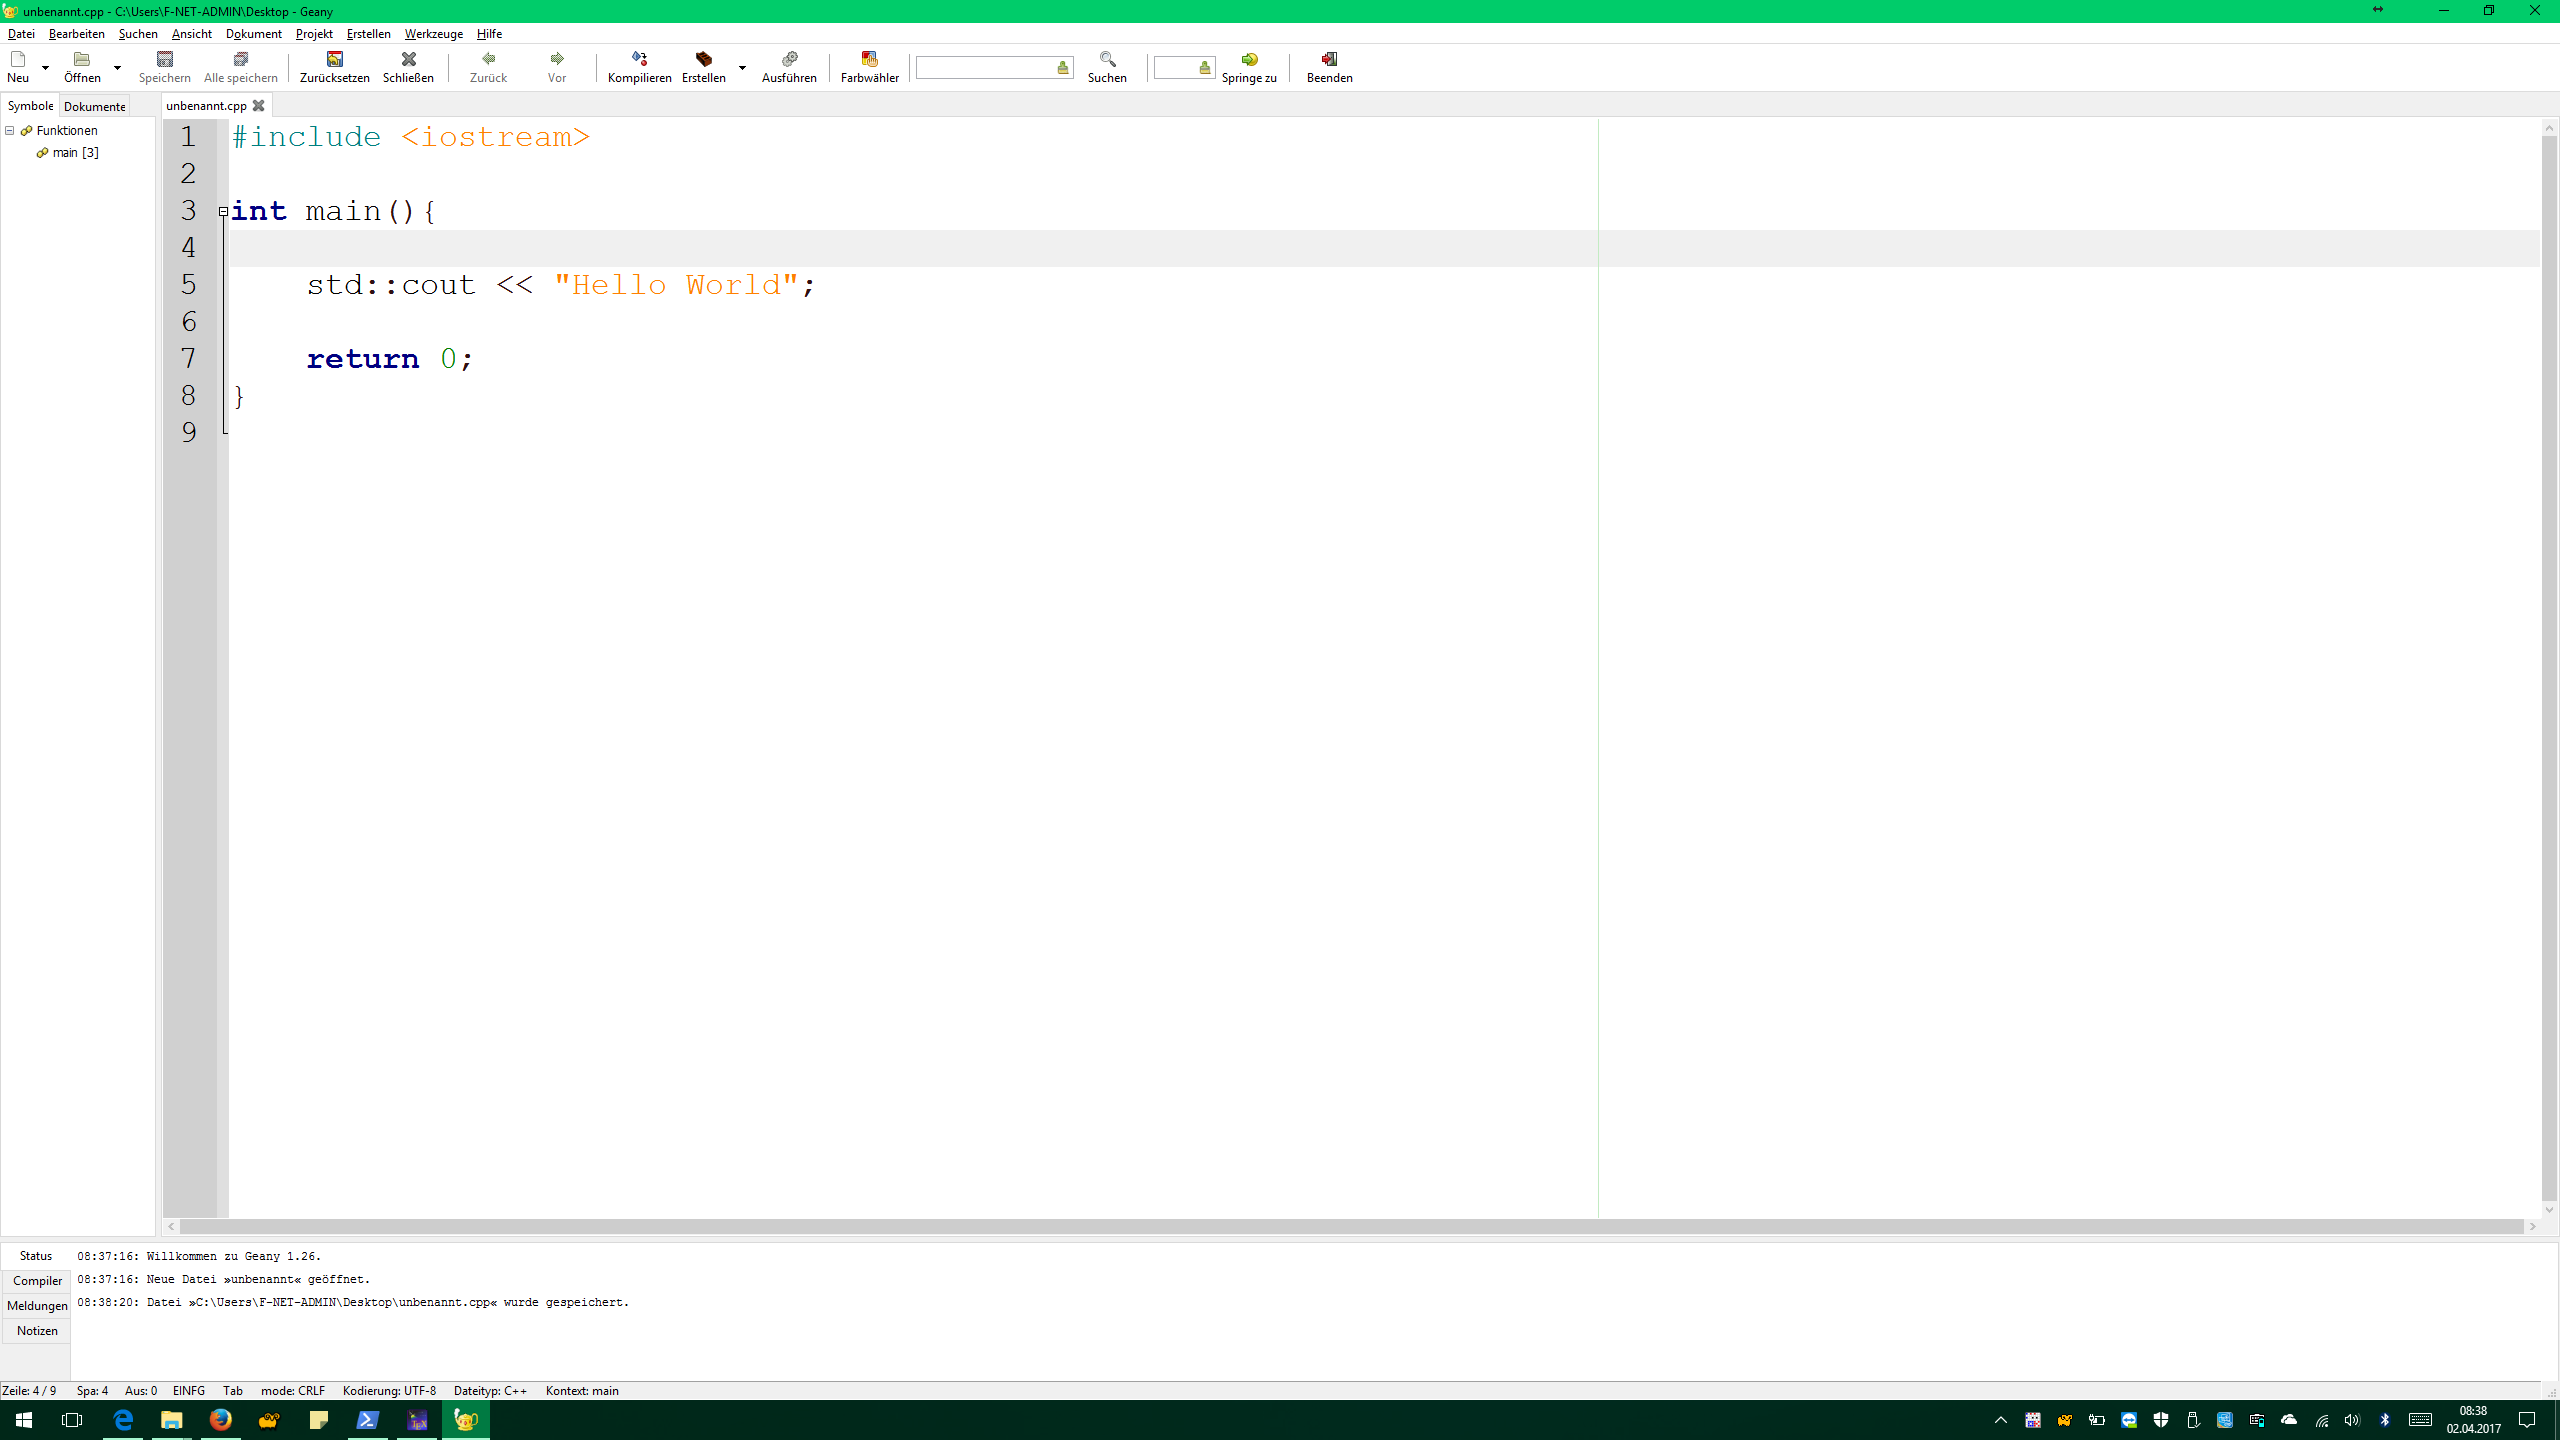
\includegraphics[width = \textwidth]{01/geany.png}
	\caption{Geany}
	\label{pic:geany}	
\end{figure}
\begin{figure}
	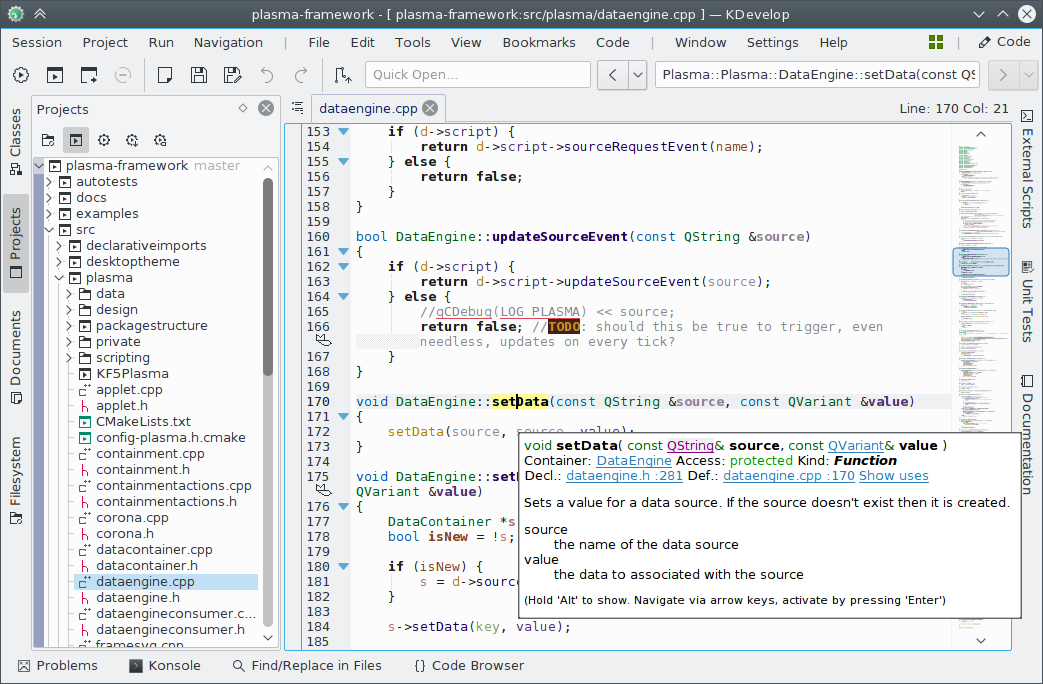
\includegraphics[width = \textwidth]{01/kdevelop.png}
	\caption{KDevelop}
	\url{https://www.kdevelop.org/sites/www.kdevelop.org/files/inline-images/kdevelop5-breeze_2.png}
	\label{pic:kdevelop}	
	\label{end:ide:picts}
\end{figure}
\end{center}

\section{Referenzen}

\begin{itemize}
	\item Buch:
	\begin{itemize}
		\item Wolf, Jürgen: C++ - Das umfassende Handbuch. Rheinwerk Computing
	\end{itemize}
	\item Websites:
	\begin{itemize}
		\item \url{http://en.cppreference.com/w/}
		\item \url{ttp://www.cplusplus.com/reference/}
	\end{itemize}
\end{itemize}
%\###### Anmerkung ergänzen (Buch)
\# Es gibt auch offline Versionen der Referenzen.
\section{The Hello World}

\subsection{Das erste kleine Programm}
\begin{tcblisting}{colback=yellow!10,colframe=yellow!40!black,listing only,
		title=Unser erstes C++ Programm, fonttitle=\bfseries}
#include <iostream>
// "Einbinden" d.h. 1-zu-1-Einfuegen des Headers iostream.h

int main(int argc, char* argv[])
// main-Funktion: Einstiegspunkt der Anwendung
// count: Anzahl der uebergebenen Parameter 
// arg: Pointer auf ein Array von Pointern auf C-Style-Strings (die Parameter)
// Parameter der main-Funktion duerfen in der Signatur auch weggelassen werden.

// Parameter der main-Funktion 
{   // Beginn vom Anweisungsblock der main-Funktion
	
	std::cout << "Hello World" << std::endl;
	// Ausgabe von "Hello World" und Zeilenumbruch
	// genauer:
	/*
	* implizite Klammerung:
	* ((std::cout) << "Hello World") << (std::endl);
	* std              ... ein Namensraum
	* ::               ... scope-Operator (Bereichsoperator)
	* cout:            ... gepufferter Standardausgabestream
	* <<               ... Ausgabeoperator (auch bitshift-Operator)
	* "Hello World"    ... C-Style-String Literal
	* endl             ... Objekt aus dem std Namensraum, das einen Zeilenumbruch ('\n') erzeugt.
	* ;                ... Abschluss einer einzelnen Anweisung
	*/
	
	for(int i = 0; i < argc; ++i ){
		std::cout << i << ". Parameter:  " << argv[i] << '\n';
	} // Beipiel fuer die Ausgabe der Komandozeilenargumente
	// argv[0] ist der Name der executable Datei
	
	return 0; // Rueckgabewert 0 "erfolgreich (ohne Fehler) beendet"
}
\end{tcblisting}
Im Falle der \texttt{main-}Funktion ist es auch möglich das \textbf{return statement} (\texttt{return 0;}) wegzulassen. Dann wird implizit 0 als Funktionswert zurückgegeben. Die Funktionssignatur der \texttt{main-}Funktion darf auch in \texttt{int main(int argc, char** argv)} geändert werden. Der erste Arrayeintrag von \texttt{argv} enthält übrigens immer einen Zeiger auf den Namen (ohne Dateiendung), unter dem das Programm abgespeichert wurde. Damit ist \texttt{argc} stets mindestens 1. 
\subsection{Ein paar Werkzeuge}
Bevor wir in Kapitel \ref{real_start} einsteigen und das gesamte (naja \textit{fast}) C++ von Grund auf kennenlernen wollen, sollten Sie noch einige nützliche Werkzeuge kennen, damit Sie neu gelernte Dinge auch ohne große Probleme ausprobieren können.
\begin{tcblisting}{colback=yellow!10,colframe=yellow!40!black,listing only,
		title=... und ein paar Hilfsmittel ..., fonttitle=\bfseries}
#include <iostream>


#define debug // Benutzung bedingter Compilierung zum Debugging

int main(int argc, char* argv[]){
	
	int zahl = 0;
	std::cout << "Wie alt bist du?\n"; // eine simple Ausgabe
	std::cin >> zahl; // eine simple Eingabe
	std::cout << "Okay!\n\n";
	
#ifndef debug 
	//folgende Zeile compiliert nicht:
	std::cout << << "In 7 Jahren bist du " << 7 + zahl << " Jahre alt." << '\n';
#endif //debug
	
	std::cout << "Tsch" << static_cast<char>(0x81) << "ss\n";
	//https://de.wikipedia.org/wiki/Codepage_850
	
	std::cin.sync();
	std::cin.get(); // warted auf Enter zum fortfahren.
	
	/*
	Das ist
	ein mehrzeiliger
	Kommentar
	*/
	
	// Das ist ein einzeiliger Kommentar.
}
\end{tcblisting}
\begin{center}
\begin{tabular}{|c|c|}
	\hline
	\textbf{Objekt} & \textbf{Funktionalität} \\
	\hline \hline
	\texttt{cin}	& Standardeingabe, standardmäßig Eingabe von Tastatur \\
	\hline
	\texttt{cout}	& (gepufferte) Standardausgabe \\
	\texttt{cerr}	& ungepufferte Standardfehlerausgabe \\
	\texttt{clog}	& gepufferte Standardfehlerausgabe \\
	\hline
	\multicolumn{2}{|p{11cm}|}{\textbf{Achtung: Diese Streamobjekte liegen alle im Namensraum \texttt{std} und werden nach einem \texttt{\#include <iostream>} erst verfügbar}}\\
	\hline
\end{tabular}
\end{center}

\subsection{Programmierstil}
Bevor es richtig losgeht, möchte ich noch ein paar Worte über den Programmierstil loswerden. Im Grunde genommen dürfen Sie Ihren C++-Code schreiben, wie sie wollen, solange Sie die Spezifikationen von c++ einhalten. Es gibt auch nicht \textit{den einen} Programmierstil, der sich durchgesetzt hat. Sie schreiben aber einen viel leserlicheren, einfacher wartbaren und für das Auge schöneren Code, wenn Sie beim programmieren \textbf{konsistent bleiben}, was einige Aspekte betrifft:
\begin{center}
	\begin{tabular}{|c||c|}
		\hline
		Einrückungen	&	tabs or spaces \\ \hline
		Anweisungen pro Zeile & eine, ... \\ \hline
		Bezeichner		&	snake\_case, camelCase, PascalCase \\
		& kurz, prägnant, aussagekräftig \\ \hline
	\end{tabular}
\end{center}
Einige IDEs können Sie sogar mehr oder weniger dabei unterstützen, in dem Sie sich um die \textbf{Quelltextformatierung} kümmern. Dies ist gerade bei Projekten mit vielen Entwicklern hilfreich, da so ziemlich effizient für einheitliches Quelltextlayout gesorgt werden kann.

\chapter{Datentypen in C++} \label{real_start}

\section{primitive Datentypen}
Zu aller erst ist es wichtig, dass Sie mit den \textbf{eingebauten Datentypen}, auch genannt \textbf{primitive Datentypen} vertraut sind. Aus diesen setzen sich dann alle höheren Datentypen wie zum Beispiel Klassen zusammen. Auch sämtliche (oftmals relativ komplexe) Klassen aus der C++ Standardbibliothek, welche Sie zunehmend immer häufiger nutzen werden, bauen im Grunde auf nichts anderem auf.

\subsection{Die Datentypen}

\subsubsection{Kategorien}
 \begin{center}
\begin{tabular}{|l|c|r|}
	\hline
	\textbf{Kategorie} & \textbf{Typen} & \textbf{Werte}\\ \hline 
	integrale Typen & \texttt{short int, int, long int, long long int} & Ganzzahlen \\ 
	integrale char Typen & \texttt{char, wchar\_t, char16\_t, char32\_t} & Zeichen (enstpricht Ganzzahlen) \\
	floating point Typen & \texttt{float, double, long double} & Gleitkommazahlen \\
	boolsche Typen & \texttt{bool} & Wahrheitswerte \\ \hline
\end{tabular}
\end{center}

\subsubsection{Größe}
\begin{center}
	\begin{tabu} {X[-2,c]|X[-3,c]|X[-2,c]|X[c]|X[c]|X[c]|X[c]|X[c]|X[c]|X[c]|}
		\tabucline{2-}
		& \textbf{Typ} & \textbf{Synonym} & \multicolumn{7}{c|}{\textbf{Größe}} \\ \tabucline{2-}
		& & & \multicolumn{7}{c|}{\textsl{Datenmodelle bzw. Programmiermodelle}} \\ \tabucline{4-} 
		%	&&&&&& WIN & Linux, Mac  \\ \tabucline{2-}
		&&& IP16 & LP32 & ILP32 & LLP64 & LP64 & ILP64 & SILP64  \\ \tabucline{2-}
		& \texttt{short int} & \texttt{short} & 16 & 16 & 16 & 16 & 16 & 16 & 64 \\ \tabucline{2-}
		& \texttt{int} & & 16 & 16 & 32 & 32 & 32 & 64 & 64 \\ \tabucline{2-}
		& \texttt{long int} & \texttt{long} & 32 & 32 & 32 & 32 & 64 & 64 & 64 \\ \tabucline{2-}
		{\tiny C++11} & \texttt{long long int} & \texttt{long long} & 64 & 64 & 64 & 64 & 64 & 64 & 64 \\ \tabucline[1.5pt]{2-}
		& \texttt{char} && \multicolumn{7}{l|}{$\geq 8$, (meist 8) } \\ \tabucline{2-}
		& \texttt{wchar\_t} && \multicolumn{7}{l|}{implementierungsabhängig: 16 oder 32) } \\ \tabucline{2-}
		& \texttt{char16\_t} && \multicolumn{7}{l|}{$\geq 16$ } \\ \tabucline{2-}
		& \texttt{char32\_t} && \multicolumn{7}{l|}{$\geq 32$ } \\ \tabucline[1.5pt]{2-}
		& \texttt{float} && \multicolumn{7}{l|}{implementierungsabhängig} \\ \tabucline{2-}		
		& \texttt{double} && \multicolumn{7}{l|}{implementierungsabhängig} \\ \tabucline{2-}		
		& \texttt{long double} && \multicolumn{7}{l|}{implementierungsabhängig} \\ \tabucline[1.5pt]{2-}
		& \texttt{bool} && \multicolumn{7}{l|}{implementierungsabhängig} \\ \tabucline{2-}		
				
	\end{tabu}
\end{center}

\subsubsection{signed and unsigned}
Die Schlüsselworte \texttt{signed} sowie \texttt{unsigned} sind nur für integrale Typen von Bedeutung. Integrale Typen sind standardmäßig \textbf{signed} und können daher sowohl \textbf{negative als auch positive Werte} annehmen. In diesem Fall erfolgt die Codierung mit dem 2er-Komplement. Man darf das Schlüsselwort \texttt{signed} auch explizit davorschreiben. Setzt man andererseits \textbf{unsigned} vor einen integralen Typ, so kann dieser nur \textbf{nichtnegative Werte} speichern, beziehungsweise seine Werte werden als solche interpretiert.

\begin{center}
\begin{tabular}{c|c}
	\textbf{signed} & \textbf{unsigned} \\ \hline
	vorzeichenbehaftete Ganzzahlen & vorzeichenlose Ganzzahlen
\end{tabular}
\end{center}
 
Eine Ausnahme bilden die char Typen: Hier ist es implementierungsabhängig, ob beispielsweise eine \texttt{char} standardmäßig als \texttt{signed char} oder als \texttt{usigned char} implemetiert ist.

\subsubsection{Wertebereiche}

\begin{center}
\begin{tabular}{|c|c|}
	\hline
	\textbf{Typen}	& \textbf{Wertebereich} \\ \hline
	\texttt{signed} Integer der Breite n bit & $-2^{n-1}, \dots , -1,0,1, \dots ,2^{n-1}-1$ \\ 
	\texttt{unsigned} Integer der Breite n bit & $0,1, \dots ,2^{n}-1$ \\\hline
	\texttt{bool} & true (1), false (0) \\ \hline
	\texttt{float} &\\%######
	\texttt{double} &\\
	\texttt{long double} & \\ \hline
	
\end{tabular}
\end{center}

Leider sind die exakten Größen der Basisdatentypen fast immer \textbf{implemtentierungsabhängig} und nicht zuverlässig voraussagbar. Um zur Compilezeit eine Prüfung der Größe eines Datentyps durchzuführen, bieten sich der \texttt{sizeof()}-Operator und \texttt{static\_assert()} an. Wenn die exakte Breite (oder eine Mindestbreite) bestimmter Typen für Sie unerlässlich sind, sollten sie mit \texttt{\#include <cstdint>} eine Bibliothek importieren, die Typen fester Breite (und vieles mehr) zur Verfügung stellt.


\subsubsection{Literale}
\begin{rail}
%\railalias{dollar}{\$}
%\railterm{dollar}
	LiteralIntegerHex : (|'-') ('0x'|'[dollar]') ('0,1,...,9,A,B,C,D,E,F' +  );
	LiteralIntegerDec : (|'-') ('0'| '1,2,...,9' (() + '0,1,...,9'));
	LiteralIntegerOct : (|'-') '0' ('0,1,...,7' +  );
	LiteralIntegerBin : (|'-') '0b' ('0,1' +  );
	%make a real $ sign #######
\end{rail}



\begin{comment}
	\begin{table}
		\centering
		\footnotesize
		\caption{Kathodenfallableiter}
		\label{tab:kathoden}
		\begin{tabular}{@{}nd{1.1}*{3}{d{1.2}}d{1.1}d{3.2}@{}}
			\toprule
			\multicolumn{1}{@{}N}{Typenbezeichnung} &
			\multicolumn{5}{N}{Spannungsschutz für Netze} &
			\multicolumn{1}{N@{}}{Preis} \\
			&
			\multicolumn{5}{N}{Leiterspannung an der Einbaustelle} \\
			\cmidrule(lr){2-6}
			&
			\multicolumn{2}{V{6.5em}}{Nicht geerdeter Sternpunkt} &
			\multicolumn{2}{V{6.5em}}{Starr geerdeter Sternpunkt} &
			\multicolumn{1}{V{4em}}{Nenn"-spannung} \\
			\cmidrule(lr){2-3}\cmidrule(lr){4-5}
			&
			\multicolumn{1}{V{4.5em}}{Normale Leiterspannung} &
			\multicolumn{1}{V{4.5em}}{Zulässiger Bereich} &
			\multicolumn{1}{V{4.5em}}{Normale Leiterspannung} &
			\multicolumn{1}{V{4.5em}}{Zulässiger Bereich} \\
			&
			\multicolumn{1}{N}{\unit{kV}} &
			\multicolumn{1}{N}{\unit{kV}} &
			\multicolumn{1}{N}{\unit{kV}} &
			\multicolumn{1}{N}{\unit{kV}} &
			\multicolumn{1}{N}{\unit{kV}} &
			\multicolumn{1}{N}{DM} \\
			\cmidrule(r){1-1}\cmidrule(lr){2-2}\cmidrule(lr){3-3}\cmidrule(lr){4-4}%
			\cmidrule(lr){5-5}\cmidrule(lr){6-6}\cmidrule(l){7-7}
			H 484--1   & 1   & 1.15 & 1.25 & 1.45 & 1   & 220.$---$ \\
			H 484--1,5 & 1.5 & 1.8  & 1.9  & 2.2  & 1.5 & 233.$---$ \\
			H 484--2   & 2   & 2.3  & 2.5  & 2.9  & 2   & 252.$---$ \\
			H 484--2,5 & 3   & 2.9  & 3.1  & 3.6  & 2.5 & 261.$---$ \\
			H 484--3   & 3.5 & 3.5  & 3.8  & 4.3  & 3   & 264.$---$ \\
			\bottomrule
		\end{tabular}
	\end{table}

	
\tikzset{
nonterminal/.style={
% The shape:
rectangle,
% The size:
minimum size=6mm,
% The border:
very thick,
draw=red!50!black!50,         % 50% red and 50% black,
% and that mixed with 50% white
% The filling:
top color=white,              % a shading that is white at the top...
bottom color=red!50!black!20, % and something else at the bottom
% Font
font=\itshape
},
terminal/.style={
% The shape:
rounded rectangle,
minimum size=6mm,
% The rest
very thick,draw=black!50,
top color=white,bottom color=black!20,
font=\ttfamily},
skip loop/.style={to path={-- ++(0,#1) -| (\tikztotarget)}}
}

{
\tikzset{terminal/.append style={text height=1.5ex,text depth=.25ex}}
\tikzset{nonterminal/.append style={text height=1.5ex,text depth=.25ex}}
}

\newcommand{\MyUnderscore}[1]{\mathord{\begin{tikzpicture}[baseline=0.0ex, line width=0.55, scale=0.13]
\draw[] (0,0) -- (#1,0);
\end{tikzpicture}}}

\begin{tikzpicture}[
>=latex,thick,
/pgf/every decoration/.style={/tikz/sharp corners},
fuzzy/.style={decorate,
decoration={random steps,segment length=0.5mm,amplitude=0.15pt}},
minimum size=6mm,line join=round,line cap=round,
terminal/.style={rectangle,draw,fill=white,fuzzy,rounded corners=3mm},
nonterminal/.style={rectangle,draw,fill=white,fuzzy},
node distance=4mm
]

\ttfamily
\begin{scope}[start chain,
every node/.style={on chain},
terminal/.append style={join=by {->,shorten >=-1pt,
fuzzy,decoration={post length=4pt}}},
nonterminal/.append style={join=by {->,shorten >=-1pt,
fuzzy,decoration={post length=4pt}}},
support/.style={coordinate,join=by fuzzy}
]
\node [support]             (start)        {};
\node [terminal]                        { \normalfont a,b,c, \dots  A,B,C, \dots  $\_$};
\node [support]             (after ui)     {};
\node [terminal]                           {.};
\node [support]             (after dot)    {};
\node [terminal]                           {digit};
\node [support]             (after digit)  {};
\node [support]             (skip)         {};
\node [support]             (before E)     {};
\node [terminal]                           {E};
\node [support]             (after E)      {};
\node [support,xshift=5mm]  (between)      {};
\node [support,xshift=5mm]  (before last)  {};
\node [nonterminal]                        {unsigned integer};
\node [support]             (after last)   {};
\node [coordinate,join=by ->] (end)        {};
\end{scope}
\node (plus)  [terminal,above=of between] {+};
\node (minus) [terminal,below=of between] {-};

\begin{scope}[->,decoration={post length=4pt},rounded corners=2mm,
every path/.style=fuzzy]
\draw (after ui)    -- +(0,.7)  -| (skip);
\draw (after digit) -- +(0,-.7) -| (after dot);
\draw (before E)    -- +(0,-1.2) -| (after last);
\draw (after E)     |- (plus);
\draw (plus)        -| (before last);
\draw (after E)     |- (minus);
\draw (minus)       -| (before last);
\end{scope}
\end{tikzpicture}


\begin{Syntaxdiagramm}
\SynVar{NO-NUMBER} \Wiederholung{}{\SynVar{ANYTHING}}

\end{Syntaxdiagramm}

	
\end{comment}



\section{Einige Operatoren}
\section{Casts}
\section{Zusammengesetzte Datentypen}
\subsection{Arrays}
\subsection{Records und Klassen}
\subsection{Containerklassen}
\section{Klassen}
\subsection{Konstruktoren}
\subsection{Vererbung}
\subsection{Polymorphie}

\chapter{Strukturierte Programmierung}
\section{Kontrollstrukturen}
\section{Funktionen}
\section{Operatoren}
\section{Modularisierung}

\chapter{Zusätzliche Features}
\section{Templates}
\section{Exceptions}
\section{Multithreading}

\end{document}
